\documentclass[floatsintext,man]{apa6}

\usepackage{amssymb,amsmath}
\usepackage{ifxetex,ifluatex}
\usepackage{fixltx2e} % provides \textsubscript
\ifnum 0\ifxetex 1\fi\ifluatex 1\fi=0 % if pdftex
  \usepackage[T1]{fontenc}
  \usepackage[utf8]{inputenc}
\else % if luatex or xelatex
  \ifxetex
    \usepackage{mathspec}
    \usepackage{xltxtra,xunicode}
  \else
    \usepackage{fontspec}
  \fi
  \defaultfontfeatures{Mapping=tex-text,Scale=MatchLowercase}
  \newcommand{\euro}{€}
\fi
% use upquote if available, for straight quotes in verbatim environments
\IfFileExists{upquote.sty}{\usepackage{upquote}}{}
% use microtype if available
\IfFileExists{microtype.sty}{\usepackage{microtype}}{}

% Table formatting
\usepackage{longtable, booktabs}
\usepackage{lscape}
% \usepackage[counterclockwise]{rotating}   % Landscape page setup for large tables
\usepackage{multirow}		% Table styling
\usepackage{tabularx}		% Control Column width
\usepackage[flushleft]{threeparttable}	% Allows for three part tables with a specified notes section
\usepackage{threeparttablex}            % Lets threeparttable work with longtable

% Create new environments so endfloat can handle them
% \newenvironment{ltable}
%   {\begin{landscape}\begin{center}\begin{threeparttable}}
%   {\end{threeparttable}\end{center}\end{landscape}}

\newenvironment{lltable}
  {\begin{landscape}\begin{center}\begin{ThreePartTable}}
  {\end{ThreePartTable}\end{center}\end{landscape}}




% The following enables adjusting longtable caption width to table width
% Solution found at http://golatex.de/longtable-mit-caption-so-breit-wie-die-tabelle-t15767.html
\makeatletter
\newcommand\LastLTentrywidth{1em}
\newlength\longtablewidth
\setlength{\longtablewidth}{1in}
\newcommand\getlongtablewidth{%
 \begingroup
  \ifcsname LT@\roman{LT@tables}\endcsname
  \global\longtablewidth=0pt
  \renewcommand\LT@entry[2]{\global\advance\longtablewidth by ##2\relax\gdef\LastLTentrywidth{##2}}%
  \@nameuse{LT@\roman{LT@tables}}%
  \fi
\endgroup}


  \usepackage{graphicx}
  \makeatletter
  \def\maxwidth{\ifdim\Gin@nat@width>\linewidth\linewidth\else\Gin@nat@width\fi}
  \def\maxheight{\ifdim\Gin@nat@height>\textheight\textheight\else\Gin@nat@height\fi}
  \makeatother
  % Scale images if necessary, so that they will not overflow the page
  % margins by default, and it is still possible to overwrite the defaults
  % using explicit options in \includegraphics[width, height, ...]{}
  \setkeys{Gin}{width=\maxwidth,height=\maxheight,keepaspectratio}
\ifxetex
  \usepackage[setpagesize=false, % page size defined by xetex
              unicode=false, % unicode breaks when used with xetex
              xetex]{hyperref}
\else
  \usepackage[unicode=true]{hyperref}
\fi
\hypersetup{breaklinks=true,
            pdfauthor={},
            pdftitle={Children's social information-seeking as an index of sensitivity to graded uncertainty},
            colorlinks=true,
            citecolor=blue,
            urlcolor=blue,
            linkcolor=black,
            pdfborder={0 0 0}}
\urlstyle{same}  % don't use monospace font for urls

\setlength{\parindent}{0pt}
%\setlength{\parskip}{0pt plus 0pt minus 0pt}

\setlength{\emergencystretch}{3em}  % prevent overfull lines


% Manuscript styling
\captionsetup{font=singlespacing,justification=justified}
\usepackage{csquotes}
\usepackage{upgreek}

 % Line numbering
  \usepackage{lineno}
  \linenumbers


\usepackage{tikz} % Variable definition to generate author note

% fix for \tightlist problem in pandoc 1.14
\providecommand{\tightlist}{%
  \setlength{\itemsep}{0pt}\setlength{\parskip}{0pt}}

% Essential manuscript parts
  \title{Children's social information-seeking as an index of sensitivity to
graded uncertainty}

  \shorttitle{Children's sensitivity to graded uncertainty}


  \author{Benjamin E. deMayo\textsuperscript{1}}

  % \def\affdep{{""}}%
  % \def\affcity{{""}}%

  \affiliation{
    \vspace{0.5cm}
          \textsuperscript{1} Stanford University  }

  \authornote{
    Correspondence concerning this article should be addressed to Benjamin
    E. deMayo, 450 Serra Mall, Stanford, CA 94305. E-mail:
    \href{mailto:bdemayo@stanford.edu}{\nolinkurl{bdemayo@stanford.edu}}
  }


  \abstract{A growing body of research shows that children between 3 and 5 years old
show an emerging ability to monitor their own epistemic uncertainty.
However, little is known about children's sensitivity to graded
uncertainty and how they adjust their information-seeking behaviors in
situations other than those of complete knowledge and complete
ignorance. Here, I investigated children's spontaneous social
information-gathering behaviors under various levels of graded category
uncertainty. Children ages 3-5 (n = 30) were asked to categorize images
of creatures which varied in their distance from two prototype images,
such that uncertainty about category membership was greater when
distance from a prototype was greater. A live eye-tracking paradigm was
used to measure children's levels of looking to the experimenter on a
trial-by-trial basis. Children looked at the experimenter at the same
rate regardless of an item's category ambiguity, suggesting that they
did not adjust their information-seeking based on graded category
uncertainty.}
  \keywords{information gathering; uncertainty monitoring; category discrimination \\

    \indent Word count: X
  }





\usepackage{amsthm}
\newtheorem{theorem}{Theorem}
\newtheorem{lemma}{Lemma}
\theoremstyle{definition}
\newtheorem{definition}{Definition}
\newtheorem{corollary}{Corollary}
\newtheorem{proposition}{Proposition}
\theoremstyle{definition}
\newtheorem{example}{Example}
\theoremstyle{definition}
\newtheorem{exercise}{Exercise}
\theoremstyle{remark}
\newtheorem*{remark}{Remark}
\newtheorem*{solution}{Solution}
\begin{document}

\maketitle

\setcounter{secnumdepth}{0}



\section{Introduction}\label{introduction}

Early in life, children are presented with a great deal of social
information from which they can learn about the world around them. They
overhear conversations, are spoken to directly, and interact with other
people nonverbally. But when do they actively seek out information from
their social partners? Specifically, do children \enquote{know what they
don't know} well enough to seek information on the basis of their own
subjective uncertainty, or do they learn more often by passively
absorbing information from other people?

While it may seem intuitive that a child will seek help from a
conversational partner when they lack enough information to make a
decision, the questions posed above are non-trivial. Prior research
which shows that children actively explore their environments and guide
their own learning processes (e.g., Schulz \& Bonawitz, 2007) is
somewhat at odds with a separate body of research that highlights young
children's deficits when it comes to monitoring their own knowledge
states and acting on their own uncertainty (e.g., Markman, 1977). In
light of this apparent tension, the current study seeks to better
understand to what degree children's information-gathering behaviors --
in this case, gaze to a knowledgeable social partner -- are driven by
the child's epistemic uncertainty. Building on prior work that suggests
that children's social gaze may be a sensitive measure of epistemic
uncertainty (Hembacher \& Frank, n.d.), this study uses a categorization
task to examine whether children's social information-gathering
behaviors are modulated by graded uncertainty.

Below, I outline research that highlights differing accounts of
children's metacognition which show that children both engage in
spontaneous information-seeking behaviors in response to epistemic
uncertainty in order to explore their environments actively and guide
their own learning, and that children also have a limited capacity to
explicitly report on their own uncertainty. I then review studies
demonstrating children's ability to seek information selectively from
social partners who could provide helpful information when uncertainty
is high.

\subsection{Uncertainty Monitoring and Active Learning in Early
Childhood}\label{uncertainty-monitoring-and-active-learning-in-early-childhood}

Prior work on children's uncertainty monitoring has yielded mixed
evidence as to whether young children can successfully recognize when
they lack information and subsequently act on this knowledge of their
own ignorance to make a decision (Sodian, Thoermer, Kristen, \& Perst,
2012). Early studies investigating metacognitive development indicated
that children's competence in assessing and acting on their own
epistemic ignorance is limited. Markman (1977) explained a card game to
first and third grade children with ambiguous language such that
understanding the object of the game was impossible without seeking
clarification. An experimenter then prompted the child to seek this
clarification with scripted statements such as \enquote{What do you
think?}, \enquote{Do you have any questions?} and \enquote{Did I tell
you everything you need to know to play the game?} In this study,
Markman found that the younger children required more prompts before
seeking out additional information, which she argues is an indication
that young elementary school children do not engage in
\enquote{constructive processing,}; that is, they process the
instructions being given by the experimenter superficially without
executing these instructions mentally, and are consequently unaware of
gaps in their own knowledge.

Similarly, Flavell, Speer, Green, August, \& Whitehurst (1981) asked
kindergarten and second-grade children to reconstruct block structures
built by a confederate based on a tape of instructions from the
confederate, which were not sufficiently clear to successfully recreate
the structure. The researchers found that older children were more
likely to indicate the need for additional clarifying information by
replaying the tape, asking questions explicitly, or generally looking
puzzled. Conversely, kindergarteners typically did not display these
behaviors. This result demonstrated that older children were more adept
at seeking information explicitly, but it also showed that younger
children were less likely to spontaneously seek information from the
environment (for example, by replaying the tape).

Rather than measure children's spontaneous information-seeking
behaviors, some more recent research has gauged children's uncertainty
monitoring capacities by asking them to report on their decision
confidence in various contexts. When asked to report confidence in their
answers on a memory task, 3-year-olds were equally confident about
correct and incorrect responses, while 4- and 5-year-olds showed a more
adult-like pattern of lower confidence for incorrect responses(Hembacher
\& Ghetti, 2014). In a perceptual identification task, 3- to 5-year-olds
reported being less confident when they provided incorrect responses,
although overall they were still overconfident (Coughlin, Hembacher,
Lyons, \& Ghetti, 2015). In order to avoid requiring a verbal response
from children, which may obscure children's capacity to reflect on their
own ignorance, these studies used a pictorial confidence scale when
prompting children to report on their uncertainty. However, the
possibility exists that even these studies underestimate children's
ability to monitor their own uncertainty because they require children
to explicitly report their confidence (even if not in an open-ended
verbal response), and that children can act on their own uncertainty
before they can communicate it through explicit responses or reflect on
it consciously.

\subsection{Children's Spontaneous Information-seeking
Behaviors}\label{childrens-spontaneous-information-seeking-behaviors}

In contrast to the explicit confidence measurements used in the studies
discussed above, some research has shown that children engage in
spontaneous information-gathering behaviors -- that is, behaviors that
are not prompted explicitly by an experimenter -- more often when they
are faced with uncertainty. These studies demonstrate that children
engage in active learning, in which the learner decides what information
they want to be exposed to, rather than having the decision made for
them by a teacher (Gureckis \& Markant, 2012). While early research on
children's metacognitive development also measured unprompted
information-seeking behaviors and found that younger children do not
engage in spontaneous information-seeking, these early studies often
required an explicit verbal response from children, as in Markman
(1977). Furthermore, studies such as Flavell, et al. (1981) showed
children's deficit in realizing when instructions are insufficient,
which may be more difficult for children than realizing they lack other
types of knowledge, such as memory of an event. Specifically, it may be
particulary difficult for children to realize they lack understanding or
knowledge of instructions, since doing so requires that children realize
that they may encounter an obstacle in the future that may not be
immediately apparent to them at the moment the instructions are given.

Recent research which at least partially alleviated these task demands
has found evidence of children's engagement in spontaneous
information-seeking. In one study, when 2-year-old children were asked
to find a sticker hidden inside of one of several tubes, they peeked
inside the tubes more when they had not seen the experimenter place the
sticker, indicating that they spontaneously sought out more information
when deprived of sufficient information to make a decision (Call \&
Carpenter, 2001). In another study, young children were shown a group of
toys that either differed in their color or in how they felt to the
touch (Robinson, Haigh, \& Pendle, 2008). All of the toys were put into
a bag by the experimenter, who mixed them up and then picked out a toy.
In the condition where the experimenter put the toy on the table and ask
the child, \enquote{Which one is it?}, children more often reached out
and touched the toy more when its distinctive quality was texture than
when it was color. In contrast, when the experimenter handed the object
to the child, thus giving the child visual and tactile access to the toy
simultaneously, children still correctly were able to identify whether
the toy was soft or hard, but unable to accurately report that they had
arrived at this conclusion by touching the toy. This result demonstrates
that children interact with the environment using sensory modalities
that will most effectively fill in gaps in uncertainty, even if they are
unable to explicitly report doing so.

Schulz and Bonawitz (2007) also found that when young children were
presented with a causally-confounded toy (i.e., a toy that exhibited a
behavior whose causal structure could not be deduced) and could choose
between playing with that toy or a novel toy, they chose to further
explore the causally-confounded toy. However, when the choice was
between continuing to play with a causally-unconfounded toy and playing
with a new toy, children preferred the novelty of exploring the new toy,
demonstrating that children play spontaneously in order to maximize
learning based on uncertainty about the world. Goupil \& Kouider (2016)
found that even preverbal infants faced with an object-retrieval task
persisted on their answers more when they were correct than incorrect,
showing that children are sensitive to their own likely accuracy and
flexibly adjust their actions accordingly.

\subsection{Children's Social Referencing and Social-Information
Gathering}\label{childrens-social-referencing-and-social-information-gathering}

Taken together, these studies provide compelling evidence that children
choose to seek more information specifically to resolve uncertainty, and
that they sample sources of evidence that are most likely to provide
disambiguating information. In this study, I examine the selectivity of
children's spontaneous sampling social information. In order to do this,
children must consider other people to be helpful sources of
information.

Evidence in a number of experimental contexts suggests that infants and
young children reference trusted adults for disambiguating information
in situations of uncertain outcomes and potential danger. Sorce, Emde,
Campos, and Klinnert (1985) showed that infants look to their mothers to
determine whether it is safe to proceed crawling over a
\enquote{visual-cliff}, a glass table that is actually safe to walk on
but which looks like a daunting drop-off to an infant. When infants'
caregivers showed an encouraging expression, infants tended to crawl
onto the glass surface, whereas they avoided doing so when their mother
showed a frightened facial expression. Other studies have shown that
children use caregivers' emotional appraisals of novel toys (Feinman,
1982; Hornik, Risenhoover, \& Gunnar, 1987; M. Klinnert, 1981) and
recently-met strangers (Feinman \& Lewis, 1983) (Feinman \& Lewis, 1983)
to inform how they interact with newly-encountered aspects of their
environments.

The above studies provide strong evidence that children, starting in the
early stages of infancy, use others' appraisals of the world around them
to disambiguate uncertainty about the safety or physical affordances of
the environment. However, there is only limited prior research that
sheds light on whether children's searches for social information are
driven by gaps in the child's knowledge and the child's own awareness of
these gaps. There are several reasons to suspect that children may be
less selective with their social information-seeking than they are with
information-seeking in non-social contexts. Some forms of social
information-seeking, such as looking at others' faces, are less costly
than other forms of manual exploration of the environment such as
tactile play, in that they may require less time and cognitive
resources. Additionally, social information may be sufficiently salient
such that children sample it regardless of the uncertainty associated
with a particular situation. This is particularly plausible given
research which demonstrates that children focus more attention to faces
and other socially informative aspects of complex scenes beginning as
early as infancy (Frank, Vul, \& Johnson, 2009; Frank, Vul, \& Saxe,
2012). Nevertheless, prior research has shown that children show
selectivity in some of their social information-gathering behaviors.
Below, I review studies that demonstrate that children are selective
when choosing their informants, and that they more heavily weight social
information in situations of uncertainty.

\subsection{Selective trust in
testimony}\label{selective-trust-in-testimony}

A large body of evidence suggests that young children are selective
social learners in terms of whom they choose as their informants.
Younger children tend to use an informant's familiarity as a cue to the
trustworthiness of the information being offered, but children gradually
shift to depend more on an informant's demonstrated competence and
expertise as they grow older (Corriveau \& Harris, 2009; Lucas, Lewis,
Pala, Wong, \& Berridge, 2013). In one study, children were found to
generally be proficient at tracking the accuracy of an informant's
information when explicitly probed. Furthermore, children who showed
this proficiency selectively learned novel object labels from an
accurate informant, while those who failed to discriminate between an
accurate and inaccurate informant likewise did not selectively use
information from the accurate informant (Koenig, Clément, \& Harris,
2004). Children also show selective learning from an informant who
appears uncertain versus one who is clearly knowledgeable, and are able
to assess someone else's knowledge on a particular topic beyond
perceptual cues such as facial expression (Sabbagh \& Baldwin, 2001).
Taken together, these studies show that children, beginning in the
preschool years, choose their information sources in order to maximize
knowledge gain. However, it remains unclear whether children are
similarly selective in their social information-gathering depending on
their own level of epistemic ignorance.

\subsection{Selective social learning on the basis of
uncertainty}\label{selective-social-learning-on-the-basis-of-uncertainty}

Despite young children's apparent lack of ability to explicitly report
their own uncertainty, a few studies indicate that young children may
seek and use information selectively from other people on the basis of
epistemic uncertainty. Tamis-LeMonda et al. (2008) extended the finding
of Sorce et al. (Sorce et al., 1985) in order to determine whether
children consider the expressions of their caregivers more when the
safety of the environment is more uncertain versus when it is completely
certain. In this study, researchers tested whether 18-month-old infants
would walk down slopes of varying risk levels when given either
encouraging or discouraging signals from their mothers. The researchers
found that children tended to ignore their mothers' encouraging messages
when faced with a slope that was clearly too steep to walk down safely,
and similarly ignored mothers' discouraging messages when the slope was
obviously safe. At borderline slopes, when it was unclear to infants
whether the slope was safe to walk down or not, children tended to
comply much more consistently with the encouragement or discouragement
provided by mother, showing that even infants selectively give more
weight to social information when perceptual input is not enough to make
a decision.

While the study by Tamis-LeMonda et al. examined children's selective
integration of social information, it did not include children's
sampling (e.g., through gaze shifts) of social information as a
dependent measure. Some recent research has begun to address the
question of whether children actively seek out information from their
social partners when uncertainty is high. Vredenburgh and Kushnir (2016)
investigated children's propensity to ask questions when faced with
toy-assembly tasks of differential levels of difficulty. They found that
preschoolers were significantly more likely to ask an experimenter for
help on tasks that were more difficult for them, indicating that
children adjust their social information-gathering behavior to optimize
their learning. Another study examined whether infants selectively
reference their social partners' gaze when their social partners has
uttered an ambiguous object label (Vaish, Demir, \& Baldwin, 2011). In
this study, infants heard an experimenter produce a novel label when
there were either two or one single objects present. Infants looked up
more at the experimenter when there were two objects present and the
referent of the experimenter's label was thus ambiguous.

A later study by Hembacher, deMayo, and Frank (2017) sought to replicate
and extend the finding of Vaish et al. with preschool-aged children. In
this study, children aged 2 - 5 were presented with either one or two
objects, heard a label produced by the experimenter, and asked to put
the labeled item in a bucket. The number of objects (1 vs.~2) and their
familiarity to the child were varied to manipulate referential
ambiguity. Across two experiments, they found that children looked up at
the experimenter more as they were making their choice when referential
ambiguity was present. Specifically, children did the most looking at
the experimenter when both objects were novel, did the least looking
when both objects were familiar, and did an intermediate amount when one
of the objects was familiar and one was novel. Additionally, when
helpful gaze from the experimenter was included as a between-subjects
manipulation, children looked up at the experimenter more when one
object was familiar and one was novel, but only when helpful gaze was
absent, suggesting that children's social referencing might be sensitive
to graded levels of epistemic uncertainty. Thus, children are not only
sensitive to states of complete ignorance and complete knowledge, but
may also be sensitive to intermediate levels of evidence for a
hypothesis.

\subsection{Sensitivity to graded
uncertainty}\label{sensitivity-to-graded-uncertainty}

Although these results provide initial evidence that children seek
social information on the basis of graded uncertainty, this study did
not manipulate ambiguity in a continuous fashion, but rather presented
children with only one intermediate level of uncertainty between
complete certainty and complete ambiguity. In many learning contexts
(i.e., category learning) many more degrees of ambiguity exist than
complete certainty and complete ambiguity.

It is unclear whether young children are sensitive to intermediate
levels of epistemic uncertainty, but some research suggests that their
capacity to monitor graded uncertainty may be limited. One body of
research has shown that children over the age of 3 can report on states
of complete ignorance or complete knowledge when asked about an object
that is being hidden (e.g., Wimmer, Hogrefe, \& Perner, 1988), meaning
that when they are asked if they know which object has been hidden, they
can accurately report on their own knowledge state if they have seen the
hiding event (complete certainty) or have not seen any objects at all
(complete ignorance). However, children of the same age struggle in
partial exposure tasks, in which they are shown two objects and told one
of them will be hidden, but are not able to see which one ends up being
hidden (Kloo \& Rohwer, 2012; Sodian \& Wimmer, 1987). In these
situations, children tend to erroneously report that they know which
object has been hidden, even though they had no visual access to the
hiding event. Some studies, however, show that children as young as 2 or
3 years old engage in spontaneous information-seeking when faced with
ambiguity in partial exposure tasks (Call \& Carpenter, 2001; Kloo,
Rohwer, \& Perner, 2017). In sum, while 3 to 6-year-old children
struggle to demonstrate explicit or verbal reasoning about their own
ignorance in partial exposure tasks, some studies demonstrate that
children may engage in spontaneous information-gathering when they lack
sufficient knowledge to make a decision.

Morgan, Laland and Harris (2015) also investigated young children's
sensitivity to graded uncertainty in a different paradigm. In their
study, the researchers asked children between the ages of 3 and 7 to
determine which of two illustrated quantities was bigger; on some
trials, the quantities were more similar to each other (i.e., the task
was more difficult) than in other trials. The children then received
feedback on their choice from a group of ten informants whose level of
consensus was manipulated as an independent variable in the experiment.
After receiving feedback the group of ten informants, children could
either stick with their initial answer or change it. Children of all
ages in the study seemed to be generally insensitive to their own
uncertainty, evidenced by the fact that they tended to stick with their
original answers regardless of the initial difficulty of the task. When
they did switch their answers, however, children were more likely to
switch to the choice of the group when consensus was high, especially
among older children. Thus, although children seemed to not adjust their
usage of social information when they faced a more ambiguous problem,
they were sensitive to the graded strength of social information when
they did decide to use it. This result may have been specific to the
task at hand: this study measured children's awareness of graded
uncertainty based on whether they were willing to break from their
original choice, a metric which may underestimate children's
metacognitive reasoning. Furthermore, the studies discussed above show
that, even before they are able to report on graded levels of epistemic
uncertainty explicitly, preschool-age children spontaneously seek
information more often in situations of greater uncertainty. Building
off these findings, the current study was uses a categorization paradigm
to determine whether children's social information-gathering is driven
by graded uncertainty.

\subsection{Current Study}\label{current-study}

Children completed a category discrimination game in which they were
introduced to two creatures, and told that each creature had a specific
box that it was supposed to live in. They were then handed a number of
images depicting creatures at various points on the perceptual continuum
between the two prototype images to which they had initially been
exposed, and were asked to put each creature in its correct box. The
critical dependent measure was the duration of children's looks to the
experimenter seated across the table from them, which I measured with an
SMI RED-n eye-tracker. I predicted that children would look longer to
the experimenter when attempting to categorize stimuli closer to the
center of the perceptual continuum. This design allowed me to examine
the degree to which children's social referencing is sensitive to graded
uncertainty.

A categorization task was used here in part because category learning is
a critical learning context in early childhood. Young children possess
many mechanisms that facilitate category learning, including sensitivity
to statistical regularities in the environment (Saffran, Aslin, \&
Newport, 1996), sensitivity towards correlations of shared attributes
among objects (Younger, 1985), and acute attention to perceptual
features such as shape (Imai, Gentner, \& Uchida, 1994). Selectively
seeking social information on the basis of graded uncertainty could be
another such mechanism that aids in children's category learning. It is
an open question whether children seek out disambiguating evidence when
there is less evidence for an object's category membership.

In this study, I introduced children to two different types of
\enquote{imaginary creatures} based on stimuli created by Havy and
Waxman (2016). These stimuli sets consisted of two different perceptual
continua, such that an image's category identity was more ambiguous as
the center of the perceptual continuum is approached. I then asked
children to categorize each image. I was interested in whether
children's looks to the experimenter would reflect graded levels of
category uncertainty, such that children would spend more time looking
at the experimenter when the target creature was closer to the center of
continuum. I predicted that children's looking would show this pattern.

Eye-tracking technology was used in this study to allow me to measure
the duration of children's looks to the experimenter with greater
precision than that afforded by hand-coding. Typically, research in
social cognition that uses eye-tracking (particularly when it involves
children) measures children's gaze patterns on a digital stimulus
display such as a television screen which shows still or moving images
(Gredebäck, Johnson, \& Hofsten, 2009). This is partially due to the
fact that live-eye tracking with both children and adults is more
difficult than conventional eye-tracking displays which use a digital
stimulus display. Nevertheless, some research suggests that social
looking behaviors may differ slightly when a participant is engaged in a
real social interaction as opposed to viewing a screen image of the same
interaction (Risko, Laidlaw, Freeth, Foulsham, \& Kingstone, 2012). One
study in particular suggests that merely the potential for social
interaction that exists with a live partner draws social gaze more than
video images of the same social partner (K. E. Laidlaw, Foulsham, Kuhn,
\& Kingstone, 2011).

Despite the methodological challenges associated with live eye tracking,
its use with children and infants is not unprecedented. This technique
has mostly been used to examine social gaze irregularities in children
with Autism Spectrum Disorder (ASD), and has been used with children of
preschool and primary school age (Falck-Ytter, Carlström, \& Johansson,
2015; Nadig, Lee, Singh, Bosshart, \& Ozonoff, 2010; Noris, Nadel,
Barker, Hadjikhani, \& Billard, 2012). At least one study has also
extended this type of eye-tracking to typically-developing infants.
Gredeback, Fikke, and Melinder examined the development of infants'
gaze-following behaviors between 2 and 8 months and using a live
eye-tracking paradigm (Gredebäck, Fikke, and Melinder (2010)). In this
study, infants began showing gaze-following behaviors between 2 to 4
months of age, and were more likely to follow the gaze of a stranger
than the gaze of their mother.

In sum, since prior research indicated that such a live eye-tracking
approach was possible, and since using an eye tracker decreases the
potential for human error involved in hand-coding, I measured gaze
shifts to a real-life social partner.

\section{Methods}\label{methods}

\subsection{Participants}\label{participants}

I recruited a sample of 30 children aged 3 to 5 at the Bing Nursery
School at Stanford University in Stanford, CA. Children were asked by
the experimenter if they wanted to play a short game during their
regularly scheduled free-play. Children were predominantly white and
Asian and generally had highly-educated parents. All children were
tested by the same experimenter and were randomly assigned to one of
four counterbalance conditions.

\subsection{Stimuli, Design and
Procedure}\label{stimuli-design-and-procedure}

\subsubsection{a) Stimuli.}\label{a-stimuli.}

Stimuli were slightly altered versions of those created by Havy and
Waxman (2016). Havy and Waxman created their stimulus sets by rendering
two novel prototype images and using Norrkross MorphX to create a
perceptual continuum of stimulus items that were different morph
combinations of the two prototypes. Since pilot testing revealed that
the current task was too easy for children when the prototypes varied in
color, we transformed them to be monochromatic blue (Figure
\ref{fig:stimuli}). The images were printed and laminated to make
rectangular cards that children could insert into one of the two boxes.

\begin{figure}

{\centering 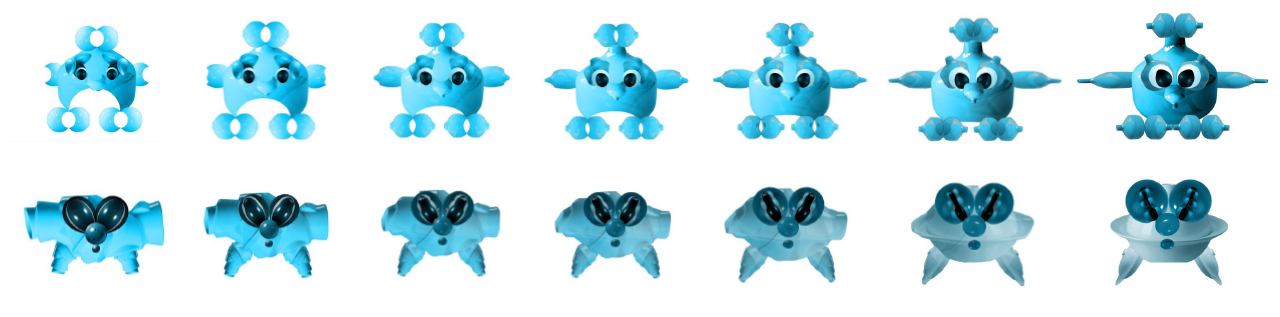
\includegraphics[width=4.27in]{../images/stimuli} 

}

\caption{Stimulus sets provided to children. Images on the ends of the spectrums are prototypes which morph into each other an a perceptual continuum.}\label{fig:stimuli}
\end{figure}

\subsubsection{b) Experimental Setup and Eye-tracking
Mechanism.}\label{b-experimental-setup-and-eye-tracking-mechanism.}

Children were seated in a small chair in front of a table which
contained two boxes, one red and one green, both placed within their
reach. The boxes had openings in the lids to allow children to deposit
the stimulus cards into them. When children entered the room, they sat
across an X-centimeter-wide table from a large poster-board which
displayed the images for the eye-tracking calibration procedure. After
the calibration phase had ended and the experimental trials began, the
poster-board was replaced with the experimenter sitting in a chair
across the table from the child.

I used an SMI REDn corneal reflection eye-tracker to measure children's
gaze shifts to the experimenter throughout the task. The eye-tracking
device was placed on two magnetic mounts in the middle of the table,
approximately X centimeters in front of the child and set an angle of X
degrees to the child's face. Critically, the eye-tracker in this case
was measuring the child's gaze shifts to the face of a real person
instead of an image on a screen. The child's field of vision was
captured by an external-viewing webcam situated directly behind and
slightly above the child's head.

\begin{figure}
\centering
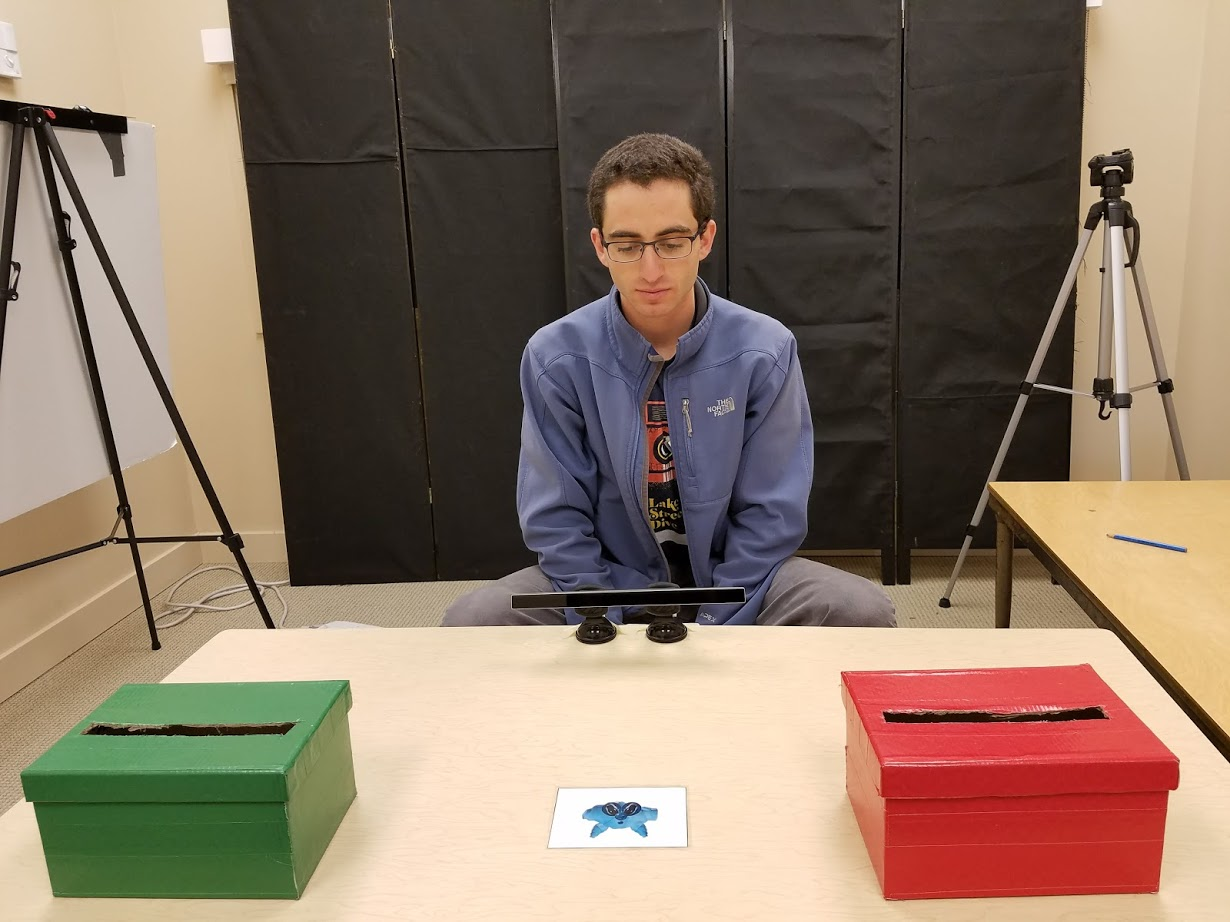
\includegraphics{../images/setup.jpg}
\caption{\label{fig:setup}Experimental setup from child's perspective. The
eye-tracker across the table recorded gaze shifts to the experimenter
throughout the task.}
\end{figure}

\begin{figure}
\centering
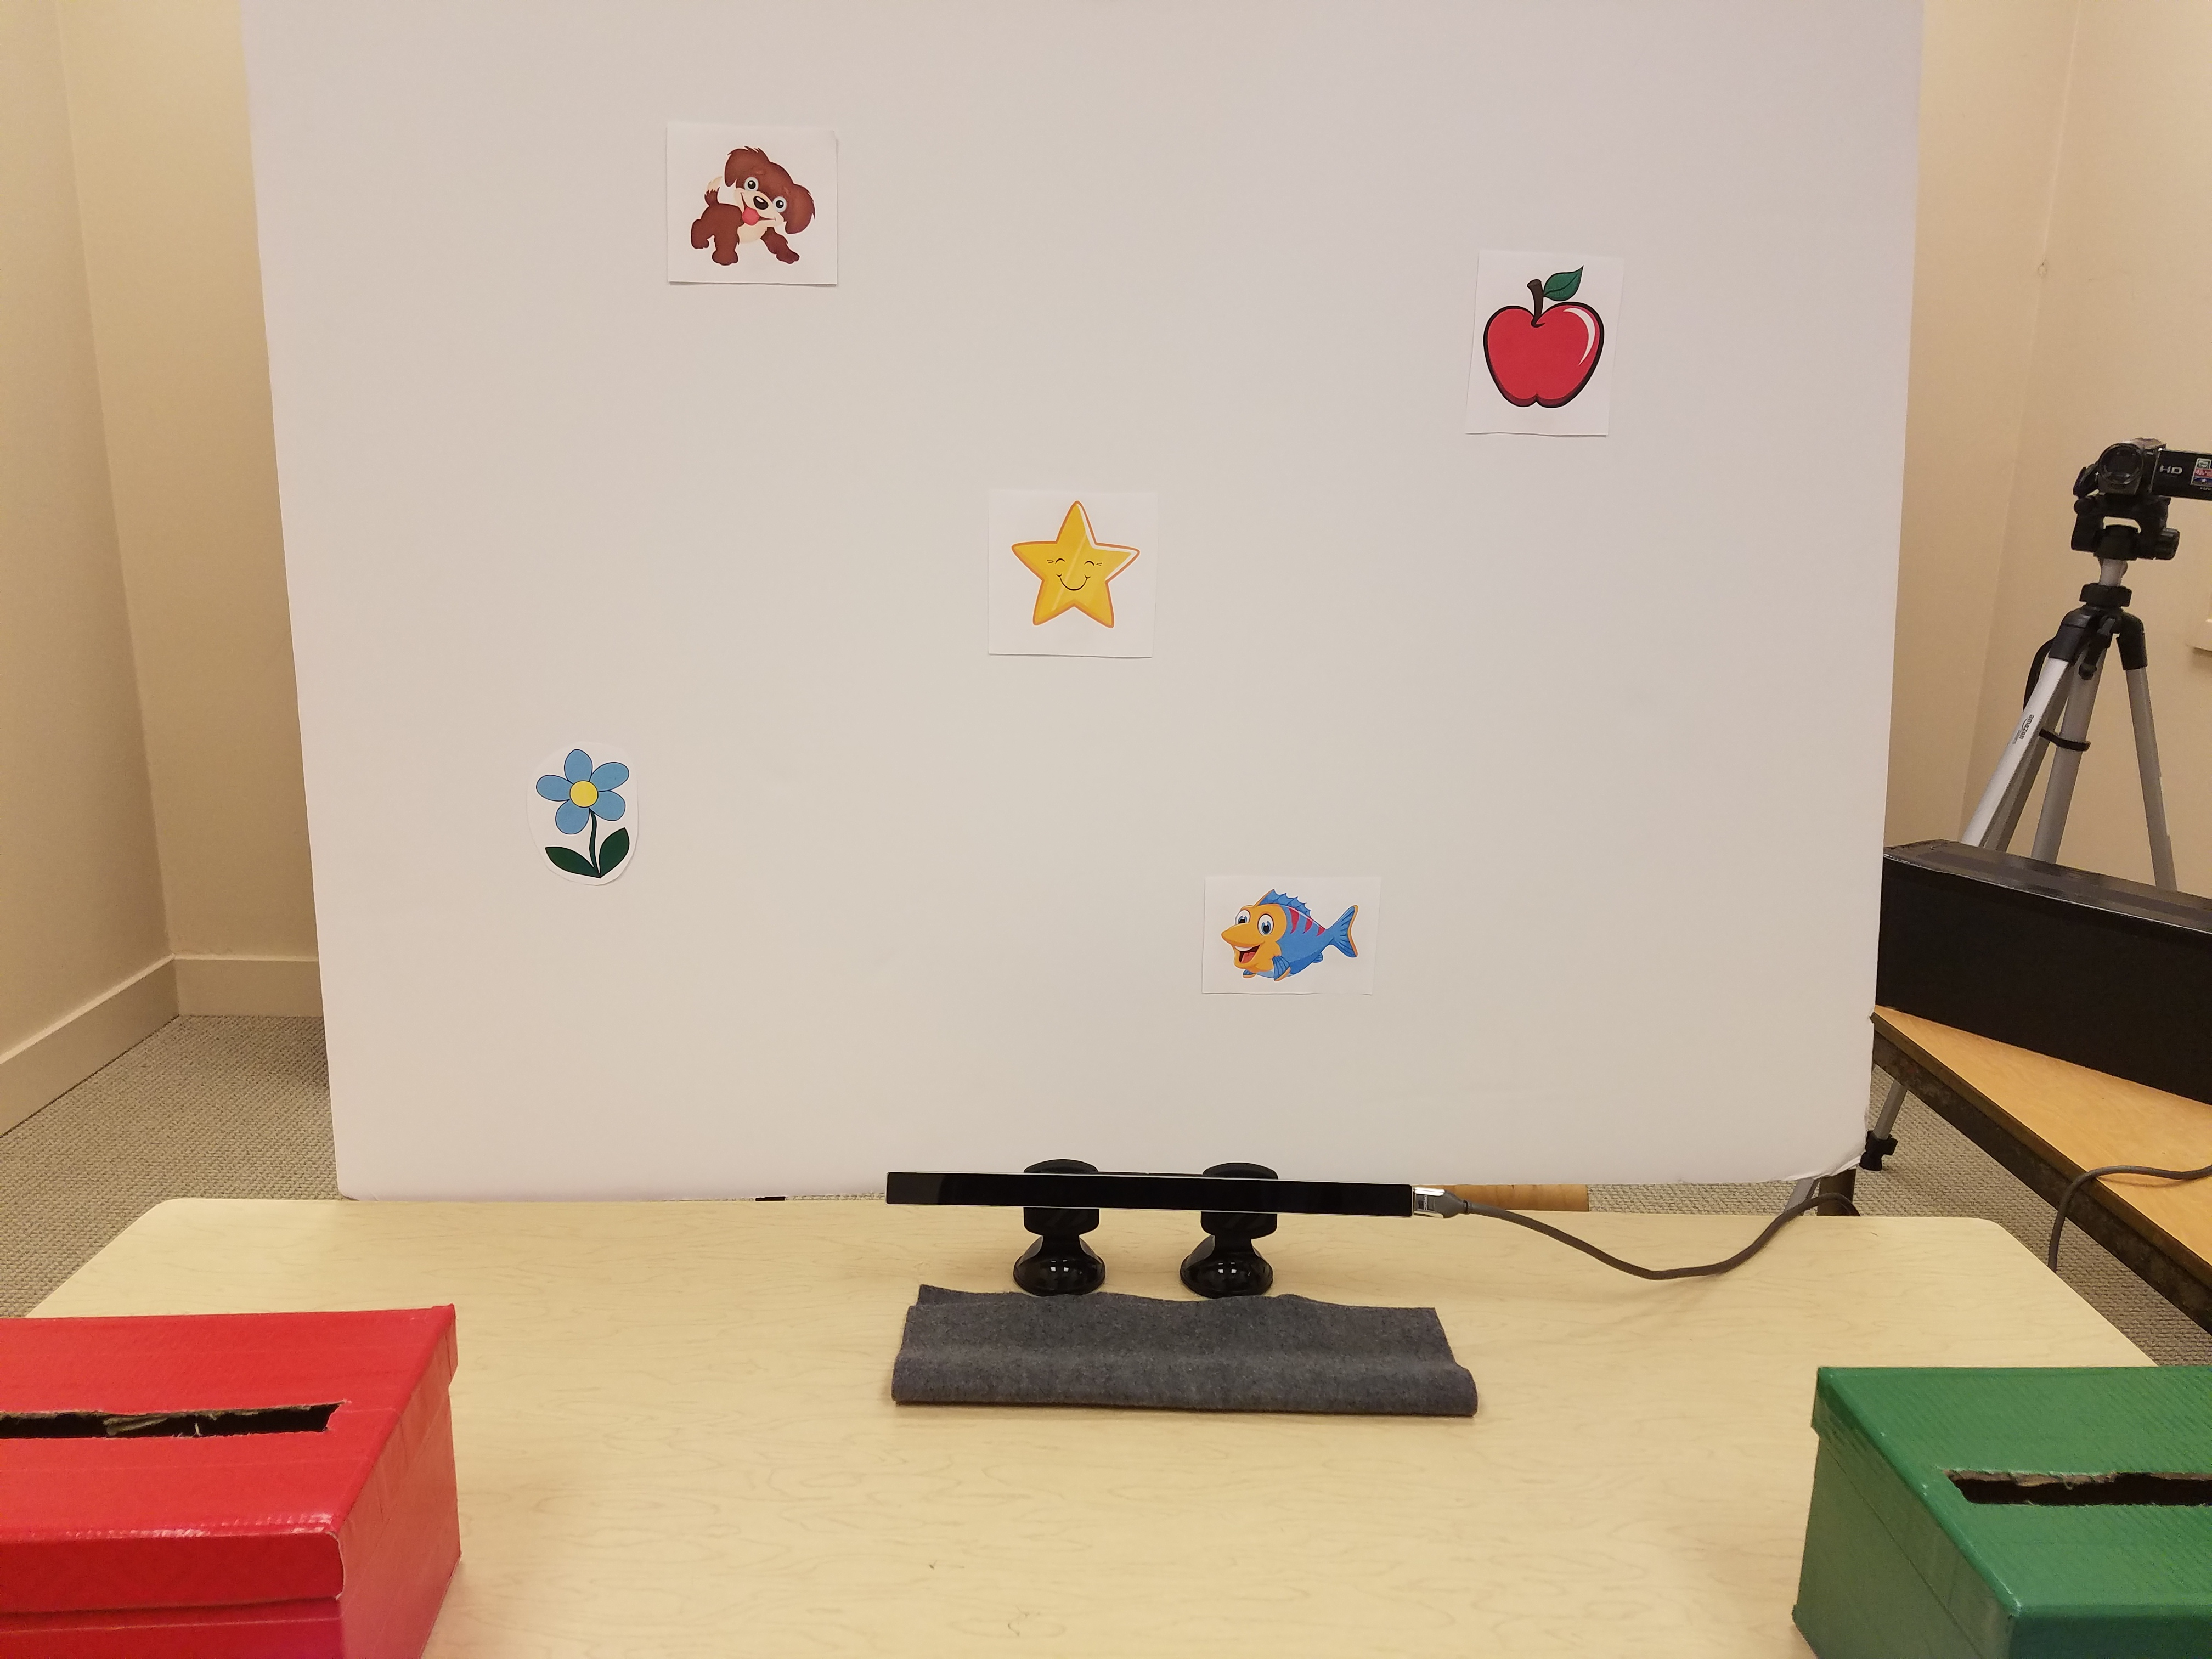
\includegraphics{../images/calibration.jpg}
\caption{\label{fig:calibration}Calibration images.}
\end{figure}

\subsubsection{c) Calibration.}\label{c-calibration.}

Children were directed to look at each of the 5 calibration images on
the poster-boarded situated across the table from them while the
experimenter approved each point one-by-one. The calibration display
consisted of a large white poster board with five cartoon images (a
smiling star, a puppy, a blue fish, a flower, and a red apple) as
illustrated in Figure \ref{fig:calibration}. After the experimenter had
approved each calibration point, the child was asked to follow the
experimenter's finger as it moved across the calibration display while
the experimenter checked to see whether the eye-tracker was accurately
representing the gaze location of the child. If the experimenter deemed
this informal test of calibration accuracy to be sufficient, the
experiment continued; if not, calibration was repeated. (Limitations of
this sort of accuracy check are addressed in the Discussion).

\subsubsection{d) Procedure.}\label{d-procedure.}

Upon entering, children were first asked to write their name on a
sticker chart that would be used throughout the task to keep them
motivated and prevent them from getting fatigued during the experiment,
which lasted about 12 minutes. After they had written their name, the
calibration phase began.

Once the calibration phase was finished, the experimenter removed the
poster board and sat across from the child. The experimenter then
explained to the child that he had brought pictures of imaginary
creatures with him, and that he needed the child's help putting them
back in their boxes. The child then categorized six practice items: two
items of a 90\% morph, two items of a 55\% morph, and two items of a
95\% morph. After the practice trials, the child completed 2 blocks of 7
test trials, each of which consisted of a 50\% morph (completely
ambiguous) and two each of 60\%, 70\%, and 100\% morphs (identical to
the prototypes). The morphs were presented in one of four pseudo-random
orders that were counterbalanced across participants. After the first
two test blocks, the child was introduced to a new pair of prototype
creatures and asked to complete the same task with these new creatures.
They then completed two new test blocks with the new set of creatures,
consisting of the same ambiguity levels as the first two test blocks. In
total, there were 6 practice and 28 test trials per child. In between
each test or practice block, children got to choose a sticker for the
chart they had made at the beginning of the experiment and were then
reminded of the two prototype creatures at each end of the perceptual
continuum. Pilot testing indicated that this procedure invoked
differential levels of accuracy based on stimulus ambiguity and avoided
performance degradation by continually re-introducing the prototypes and
offering a motivational reward after each block of 7 trials.

\subsubsection{Analysis}\label{analysis}

Each session was videotaped on a camera behind the experimenter's seat,
allowing for view of the entire experimental setup. Accuracy and trial
onsets and offsets were hand-coded using DataVyu software
(\texttt{http://datavyu.org}). A trial was defined as the span of time
between when the stimulus item became available to the child (i.e., the
experimenter let go of it) and when the item was deposited in a box. All
stimuli, data, and analyses are available at
\texttt{https://github.com/benjamindemayo/soc\_ref\_category}.

\section{Results}\label{results}

\subsection{Procedural and Manipulation
checks}\label{procedural-and-manipulation-checks}

\begin{figure}
\centering
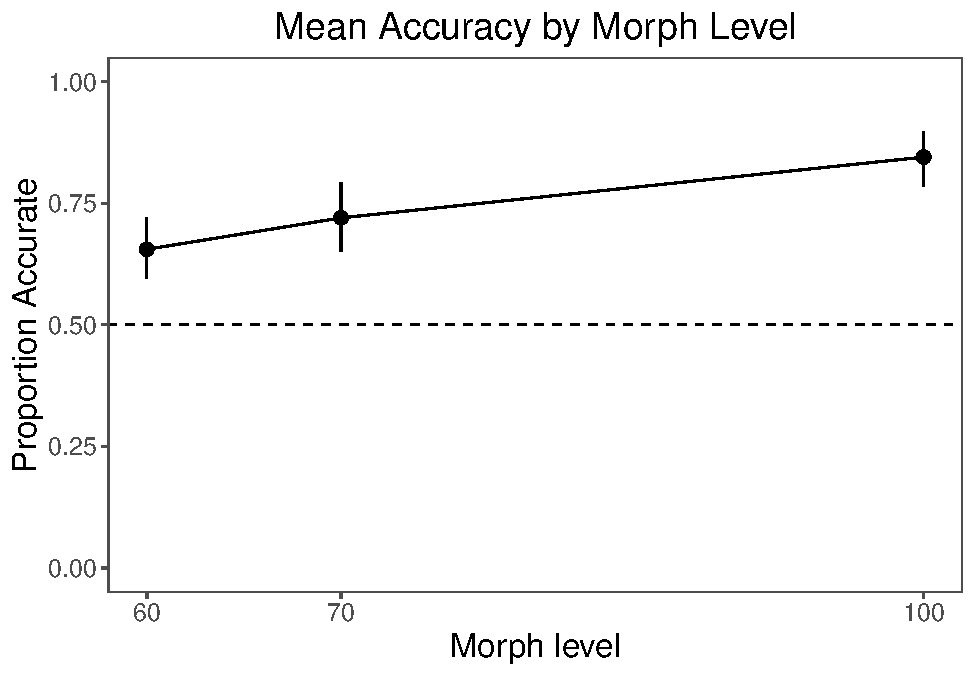
\includegraphics{soc_ref_category_paper_files/figure-latex/morphaccuracy-1.pdf}
\caption{\label{fig:morphaccuracy}Categorization accuracy for each morph
level. Error bars are 95 percent confidence intervals.}
\end{figure}

\begin{figure}
\centering
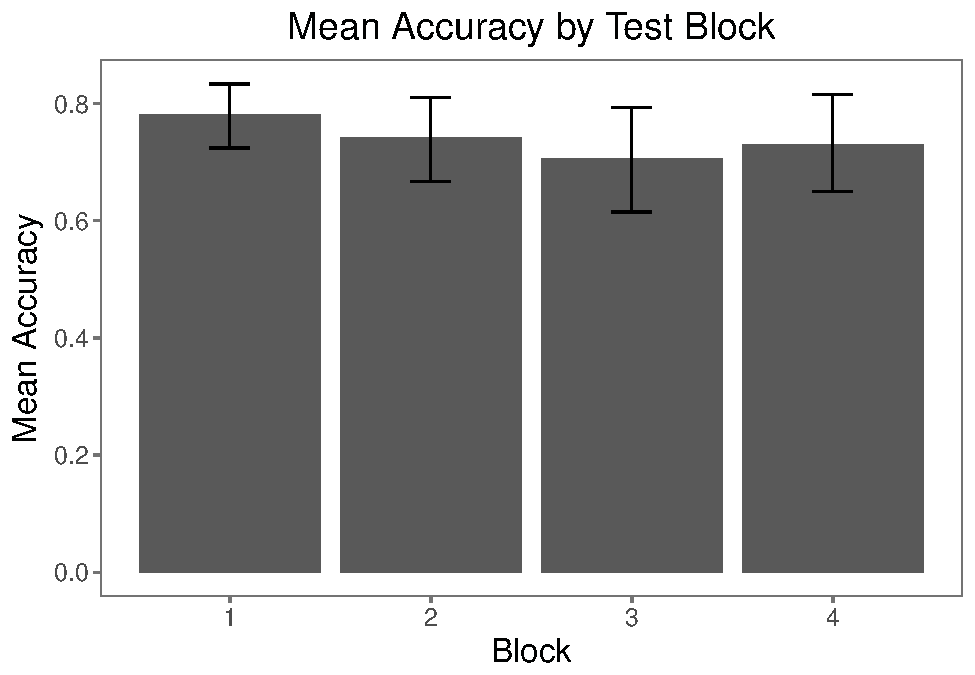
\includegraphics{soc_ref_category_paper_files/figure-latex/blockaccuracy-1.pdf}
\caption{\label{fig:blockaccuracy}Categorization accuracy for each of four
experimental blocks, suggesting that children's accuracy did not degrade
throughout the task. Error bars are 95 percent confidence intervals.}
\end{figure}

To validate the manipulation of category ambiguity in my procedure, I
first examined whether children's accuracy on the categorization task
(i.e., whether they put each item in the correct box) corresponded to
the category ambiguity of each stimulus item (Figure
\ref{fig:morphaccuracy}). Evidence from pilot testing indicated that
children's accuracy on the task was highest for the least ambiguous
stimuli, while children were least accurate when categorizing most
ambiguous stimuli. To confirm this finding of the effect of morph level
on accuracy,I used the following logistic regression model, which
accounted for random effects (such as participant and trial number):
\texttt{accuracy\ \textasciitilde{}\ morph\ *\ centered\ age\ +\ (morph\ \textbar{}\ participant)\ +\ (1\ \textbar{}\ trial)}.
I found a significant difference in children's accuracy on trials of
morph level 60 and trials of morph level 100 (\(\beta\) = 1.25, \emph{p}
\textless{} .001`). The difference in accuracy between trials of morph
level 60 and trials of morph level 70 trended towards, but did not
reach, significance, \(\beta\) = 0.40, \emph{p} = 0.09. These results
demonstrate that the task was more difficult for children when they were
tasked with categorizing more ambiguous stimuli. Children's performance
on the task also remained consistent throughout the approximately 6
minute duration of test trials (Figure \ref{fig:blockaccuracy}),
indicating that children remained engaged and motivated throughout the
experiment.

\begin{figure}
\centering
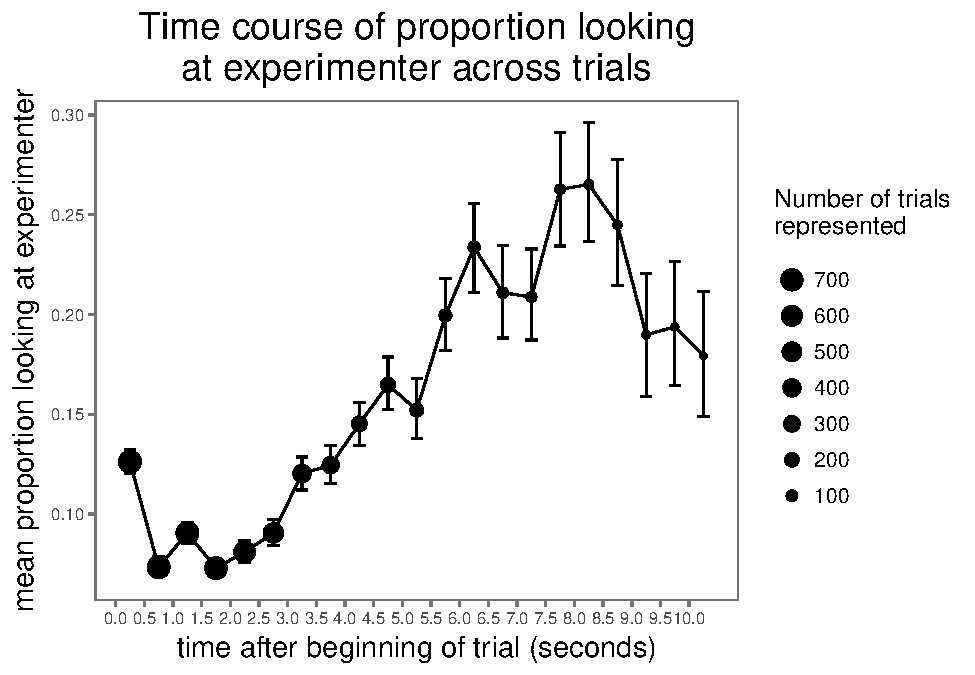
\includegraphics{soc_ref_category_paper_files/figure-latex/forwardtimecourse-1.pdf}
\caption{\label{fig:forwardtimecourse}Timecourse of proportion looking at
experimenter, in half-second intervals. Size of points indicates amount
of trials represented in each point. Error bars are 95 percent
confidence intervals.}
\end{figure}

Since this analysis method required the integration of data acquired
from various devices, I examined the average timecourse of children's
looking patterns during trials to ensure that data output from these
devices was aligning appropriate. Figure \ref{fig:forwardtimecourse}
shows, for each half-second interval after the beginning of the trial,
the average proportion of that interval that children spent looking at
the experimenter. Since the eye-tracking data collection method in this
paradigm was coarse, any looks captured by the eye-tracker were
considered to be a look in the general direction of the experimenter;
thus, the \enquote{Area of Interest} in this design was defined as the
entire spatial area for which the eye-tracker was calibrated.

\begin{figure}
\centering
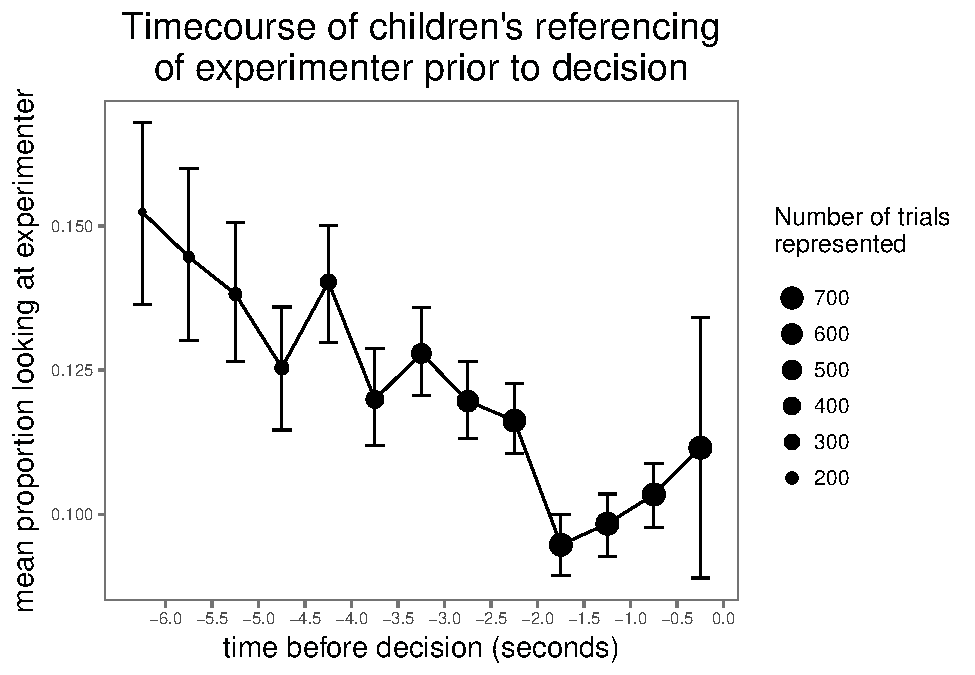
\includegraphics{soc_ref_category_paper_files/figure-latex/reversetimecourse-1.pdf}
\caption{\label{fig:reversetimecourse}Timecourse of children's looking at
experimenter prior to decision, in half-second intervals. Size of points
represents amount of trials included in each data point. Error bars are
95 percent confidence intervals.}
\end{figure}

In general, Figure \ref{fig:forwardtimecourse} shows that children tend
to look slightly more at the experimenter at the very beginning of the
trial, perhaps since this is when they are receiving the stimulus item
from the experimenter. As trial length increases, so does the proportion
of time in each half-second interval that children spend looking at the
experimenter, which may be in part because longer trials frequently
featured children asking questions and thus making eye-contact with the
experimenter. Figure \ref{fig:reversetimecourse} shows the timecourse of
children's looking in half-second intervals before the end of the trial,
which corresponds to the child's decision to place the stimulus item in
one box or another. This plot shows a peak in children's looking
behavior approximately 2.5 - 3 seconds before a decision, which is
slightly after the beginning of the trial (median trial length = 3.20
seconds). Taken together, these plots show a plausible timecourse of
children's looking throughout trials which lends confirmatory evidence
that data from various devices was integrated and aligned correctly.

\subsection{Proportion of trial looking by
morph}\label{proportion-of-trial-looking-by-morph}

Did children selectively seek out more social information when trying to
categorize more ambiguous stimulus items? I fit the data to a linear
mixed-effects model to quantify the effect of category ambiguity on
proportion of trial spent looking at the experimenter, along with any
possible developmental trends. I ran a linear mixed-effects model with
the following preregistered structure:
\texttt{proportion\ of\ trial\ spent\ looking\ \textasciitilde{}\ morph\ *\ centered\ age\ +\ (morph\ \textbar{}\ participant)\ +\ (1\ \textbar{}\ trial)}.
This model allowed me to quantify the effects of fixed factors and
random factors, including child participants and individual stimulus
items. Random effects are denoted in parentheses.

I found no significant effects of stimulus ambiguity or children's
centered age in months on the proportion of trial that children spent
looking at the experimenter (all \emph{p}-values for fixed effects
\textgreater{} 0.10), indicating that children did not selectively look
longer at the exprimenter when faced with making a more uncertain
decision.

\begin{figure}
\centering
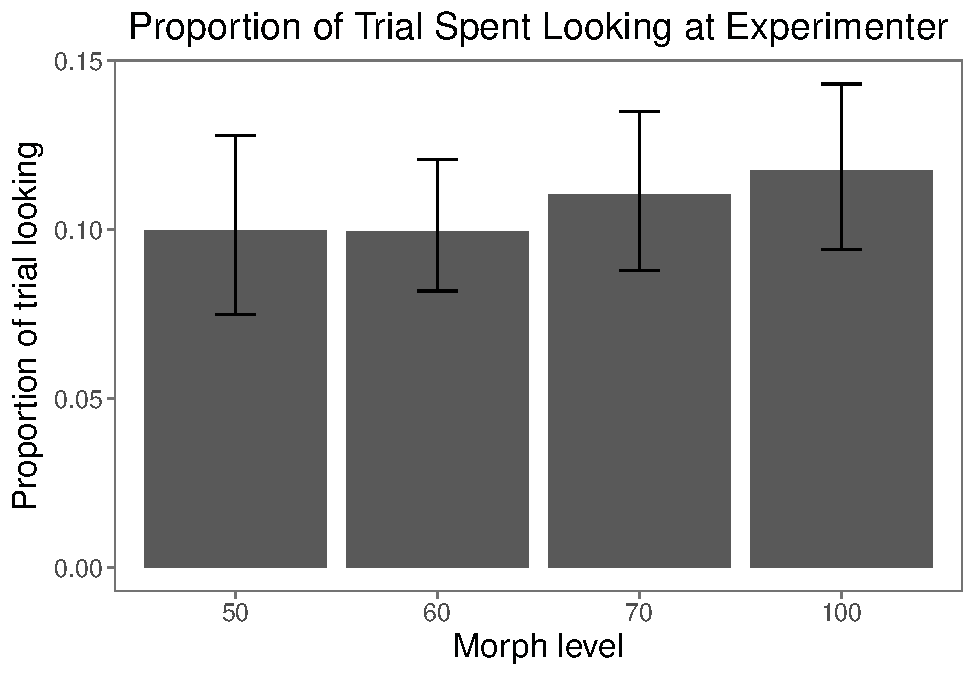
\includegraphics{soc_ref_category_paper_files/figure-latex/morphlooking-1.pdf}
\caption{\label{fig:morphlooking}Proportion of trial time spent looking at
experimenter by morph level. Error bars are 95 percent confidence
intervals.}
\end{figure}

\begin{figure}
\centering
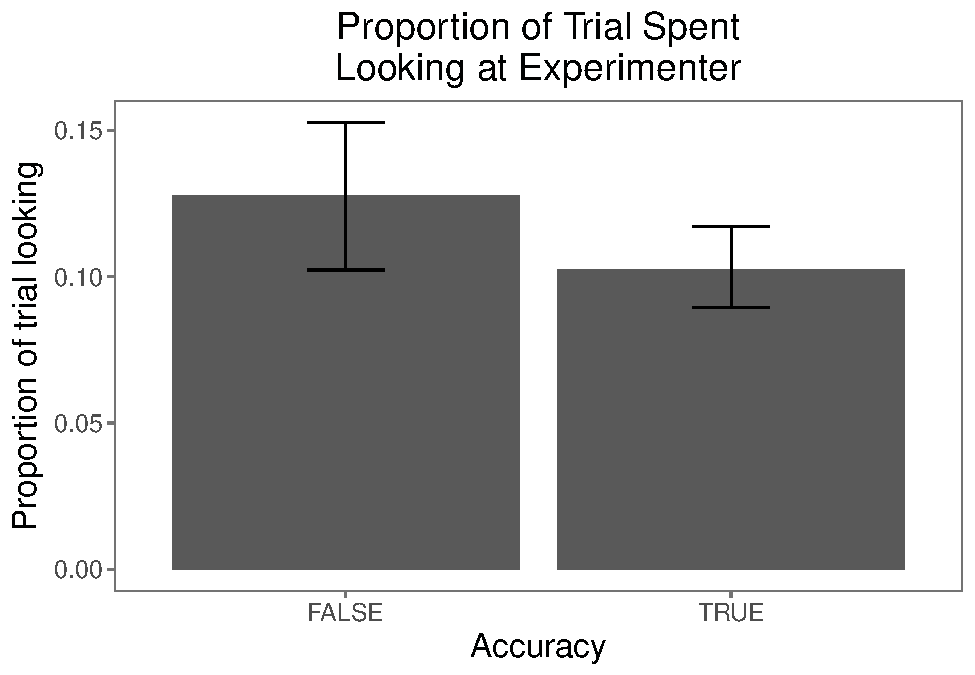
\includegraphics{soc_ref_category_paper_files/figure-latex/accuracylooking-1.pdf}
\caption{\label{fig:accuracylooking}Proportion of trials spent looking at
experimenter by children's category accuracy. Error bars are 95 percent
confidence intervals.}
\end{figure}

\subsection{Proportion of trial looking by task
accuracy}\label{proportion-of-trial-looking-by-task-accuracy}

I also examined whether children's accuracy on the task had an effect on
the proportion of trials spent looking at the experimenter (Figure
\ref{fig:accuracylooking}). To answer this question, I used a linear
mixed-effects model with the following structure, with random effects
denoted in parentheses:
\texttt{proportion\ of\ trial\ spent\ looking\ \textasciitilde{}\ accuracy\ *\ centered\ age\ +\ (accuracy\ \textbar{}\ participant)\ +\ (1\ \textbar{}\ trial)}.
I found no effect of accuracy on proportion of trials spent looking at
the experimenter (\emph{p} = 0.31), indicating that children did not
look at the experimenter more on trials when they were inaccurate versus
inaccurate.

\section{Discussion}\label{discussion}

In this study, I set out to understand whether children are sensitive to
graded levels of uncertainty, and whether they would adjust their
social-information seeking on the basis of this uncertainty. Previous
research had suggested that children explore environments in order to
maximize their learning about the world (Schulz \& Bonawitz, 2007), that
they have a limited but emerging capacity to monitor epistemic states
and uncertainty (Coughlin et al., 2015; Hembacher \& Ghetti, 2014), and
that they selectively seek out information from people who they deem to
be knowledgeable and helpful in the immediate learning context (Kushnir,
Vredenburgh, \& Schneider, 2013; Vredenburgh \& Kushnir, 2016).
Empirical evidence also suggested that children may possess some
sensitivity to graded evidence and intermediate levels of uncerainty in
the environment, in such contexts as \enquote{partial exposure} tasks
(Call \& Carpenter, 2001; Kloo et al., 2017) and word learning
situations (Hembacher \& Frank, n.d.). Thus, I hypothesized that
children would show a looking pattern that would indicate sensitivity to
graded uncertainty, and would selectively seek more social information
on trials in which they were tasked with categorizing more ambiguous
stimuli.

Contrary to my hypothesis, I found that children did not differentiate
between trials of different morph levels in their levels of looking. A
linear mixed-effects model demonstrated that stimlus ambiguity had no
effect at any level of ambiguity on the proportion of each trial that
children spent looking at the experimenter. Thus the data do not
explicitly show that children possess sensitivity to graded levels of
uncertainty, nor do they show that children strategically adjust the
amount of social information they seek out on the basis of subjective
uncertainty. Interestingly, I found no difference in looking behaviors
even between trials which were completely ambiguous (morph level 50) and
trials which were identical to the prototypes shown to children at the
beginning of each experimental block (morph level 100). This result is
particularly striking given that children were significantly less
accurate in categorizing more ambiguous items, indicating that task
difficulty was not uniform across trials. This finding contrasts that of
Hembacher, deMayo, and Frank (n.d.), who found that, in a word-learning
task, children's social information gathering was closely linked to
referential ambiguity. What might be the origin of the discrepancy
between these two findings?

One possibility is that this task, even during the most unambiguous
trials, was more challenging for children, since the task required
keeping the protoype images and their correct locations in memory. Thus,
even though children's differential levels of accuracy on the various
trial types indicate that the task was not uniformly difficult across
all trials, it may have been too demanding throughout all the trials to
be able to invoke a pattern of differential looking. Another possibility
is that the task proceeded too swiftly to facilitate children's looking
at the experimenter during individual trials. Other studies that have
measured children's visual solicitations for social information (e.g.,
Vaish et al., 2011) have measured children's looking patterns over
longer spans of time, whereas my design measured children's looking
patterns during trials that had a median length of 3.20 seconds. Below,
I discuss methodological limitations of the current work that may have
impacted my ability to detect an effect of graded category ambiguity on
children's social information-gathering.

\subsection{Limitations}\label{limitations}

The current work has several limitations that should encourage caution
against interpreting this null result as an indication of children's
inability to monitor graded levels of category uncertainty and seek out
social information accordingly. First and foremost, my data collection
method -- the use of an eye-tracker to measure children's gaze patterns
in a live person-to-person interaction -- provided coarse data. This
type of eye-tracking method is challenging to execute because it
requires children to be very still during an extended calibration phase,
and is particularly sensitive to children's body movements and any small
fluctuations in the experimental setup. Future work should strive for
greater precision from this type of data-collection method. Furthermore,
as mentioned above, this task moved quickly; a task that proceeds a
slower pace may be optimize the researcher's ability to detect an effect
of category ambiguity on children's social gaze patterns.

Additionally, it is not possible to know with complete certainty what
type of information children were seeking or expecting when they shifted
their gaze to the experimenter. We operate under the assumption that
children's foremost reason for looking was a search for disambiguating
information, but children may also have looked at the experimenter
because they were expecting a certain action (i.e., being handed the
next item in the game), asking a question unrelated to their own
uncertainty, or were simply compelled to look at their social partner
because faces are interesting to look at.

Finally, this study was performed with a convenience sample of children
from a preschool in an upper-middle/upper class neighborhood consisting
of mostly white and Asian families. Since this sample is not
demographically representative of the broader population, it is possible
that some of the eye-gaze patterns I observed were sample-specific,
given that eye contact between social partners has been shown to be
modulated by cultural norms (Akechi et al. (2013)). Nevertheless, the
preschool from which I recruited this sample makes a concerted effort to
reach out to underrepresented families in order to maintain a diverse
classroom environment.

\subsection{Conclusion and Future
Work}\label{conclusion-and-future-work}

The results of the current study do not provide a conclusive answer to
the question I posed at the outset of whether children are sensitive to
graded levels of uncertainty and adjust their social
information-gathering according to this uncertainty. Contrary to my
initial hypothesis, children did not show differential levels of looking
to the experimenter when categorizing items whose category ambiguity
varied along a spectrum. However, this could have been a task-specific
result given the pace and difficulty of the procedure children were
being asked to complete. Future work can improve on this design by
allowing for a larger temporal observation window through which to gauge
children's social-information gathering, removing some of the memory
demands present throughout this task to exagerrate the difference
between \enquote{difficult} and \enquote{easy} trial items, and by
implementing a method of tracking gaze to a social partner in a more
precise manner than what was achieved here.

In sum, the current work illustrates that, in a category-discrimination
context, children do not show obvious signs of adjusting their
social-information gathering behaviors on the basis of graded
uncertainty. However, the possibility still exists that children do
possess a sensitivity to intermediate levels of category ambiguity, and
would show this sensitivity in different contexts. This study therefore
provides a theoretical and methodological framework from which other
researchers can expand in order to better understand the development of
children's uncertainty monitoring and social information-seeking in
early childhood.

\begin{center}\rule{0.5\linewidth}{\linethickness}\end{center}

\section{Acknowledgements}\label{acknowledgements}

First and foremost, thanks to my advisors in the Stanford Department of
Psychology, Emily Hembacher and Mike Frank. They have invested so much
time, patience and energy in my personal and intellectual growth, and I
appreciate it deeply.

Thanks to my participants and their families from the Bing Nursery
School (Stanford, CA) and the Children's Discovery Museum (San Jose,
CA). Special thanks also to the Bing Nursery School teaching staff and
administration: Chia-wa Yeh, Beth Wise, Jennifer Winters, Nandini
Bhattacharjya, Jenna Rist, Nikki Baumgart, Sadie Parrinello, Jessica
Barajas, Seleena Vinayraj, Maryam Saqib, Todd Erickson, Vanessa Ibarra,
Andrea Fewster, Liz Prives, Kathryn Carruthers, and Frannie McCarthy.

Thanks to Danielle Kellier for providing helpful technical support,
advice and troubleshooting, and to Grace Bennett-Pierre and Mika Asaba
from the Social Learning Lab at Stanford for lending materials.

Lastly, a warm thanks to my parents Bob and Celia and brother Jimmy for
supporting me through all of the challenges this project has brought.

This work was funded by a Major Grant from Stanford Undergraduate
Advising and Research (UAR).

\newpage

\section{References}\label{references}

\setlength{\parindent}{-0.5in} \setlength{\leftskip}{0.5in}

\hypertarget{refs}{}
\hypertarget{ref-akechi2013attention}{}
Akechi, H., Senju, A., Uibo, H., Kikuchi, Y., Hasegawa, T., \& Hietanen,
J. K. (2013). Attention to eye contact in the west and east: Autonomic
responses and evaluative ratings. \emph{PLoS One}, \emph{8}(3), e59312.

\hypertarget{ref-call2001apes}{}
Call, J., \& Carpenter, M. (2001). Do apes and children know what they
have seen? \emph{Animal Cognition}, \emph{3}(4), 207--220.

\hypertarget{ref-corriveau2009choosing}{}
Corriveau, K., \& Harris, P. L. (2009). Choosing your informant:
Weighing familiarity and recent accuracy. \emph{Developmental Science},
\emph{12}(3), 426--437.

\hypertarget{ref-coughlin2015introspection}{}
Coughlin, C., Hembacher, E., Lyons, K. E., \& Ghetti, S. (2015).
Introspection on uncertainty and judicious help-seeking during the
preschool years. \emph{Developmental Science}, \emph{18}(6), 957--971.

\hypertarget{ref-falck2015eye}{}
Falck-Ytter, T., Carlström, C., \& Johansson, M. (2015). Eye contact
modulates cognitive processing differently in children with autism.
\emph{Child Development}, \emph{86}(1), 37--47.

\hypertarget{ref-feinman1982social}{}
Feinman, S. (1982). Social referencing in infancy. \emph{Merrill-Palmer
Quarterly (1982-)}, 445--470.

\hypertarget{ref-feinman1983social}{}
Feinman, S., \& Lewis, M. (1983). Social referencing at ten months: A
second-order effect on infants' responses to strangers. \emph{Child
Development}, 878--887.

\hypertarget{ref-flavell1981development}{}
Flavell, J. H., Speer, J. R., Green, F. L., August, D. L., \&
Whitehurst, G. J. (1981). The development of comprehension monitoring
and knowledge about communication. \emph{Monographs of the Society for
Research in Child Development}, 1--65.

\hypertarget{ref-frank2009development}{}
Frank, M. C., Vul, E., \& Johnson, S. P. (2009). Development of infants'
attention to faces during the first year. \emph{Cognition},
\emph{110}(2), 160--170.

\hypertarget{ref-frank2012measuring}{}
Frank, M. C., Vul, E., \& Saxe, R. (2012). Measuring the development of
social attention using free-viewing. \emph{Infancy}, \emph{17}(4),
355--375.

\hypertarget{ref-goupil2016infants}{}
Goupil, L., Romand-Monnier, M., \& Kouider, S. (2016). Infants ask for
help when they know they don't know. \emph{Proceedings of the National
Academy of Sciences}, \emph{113}(13), 3492--3496.

\hypertarget{ref-gredeback2010development}{}
Gredebäck, G., Fikke, L., \& Melinder, A. (2010). The development of
joint visual attention: A longitudinal study of gaze following during
interactions with mothers and strangers. \emph{Developmental Science},
\emph{13}(6), 839--848.

\hypertarget{ref-gredeback2009eye}{}
Gredebäck, G., Johnson, S., \& Hofsten, C. von. (2009). Eye tracking in
infancy research. \emph{Developmental Neuropsychology}, \emph{35}(1),
1--19.

\hypertarget{ref-gureckis2012self}{}
Gureckis, T. M., \& Markant, D. B. (2012). Self-directed learning: A
cognitive and computational perspective. \emph{Perspectives on
Psychological Science}, \emph{7}(5), 464--481.

\hypertarget{ref-havy2016naming}{}
Havy, M., \& Waxman, S. R. (2016). Naming influences 9-month-olds'
identification of discrete categories along a perceptual continuum.
\emph{Cognition}, \emph{156}, 41--51.

\hypertarget{ref-hembacherchildren}{}
Hembacher, E., \& Frank, M. C. (n.d.). Children's social referencing
reflects sensitivity to graded uncertainty.

\hypertarget{ref-hembacher2014don}{}
Hembacher, E., \& Ghetti, S. (2014). Don't look at my answer: Subjective
uncertainty underlies preschoolers' exclusion of their least accurate
memories. \emph{Psychological Science}, \emph{25}(9), 1768--1776.

\hypertarget{ref-hornik1987effects}{}
Hornik, R., Risenhoover, N., \& Gunnar, M. (1987). The effects of
maternal positive, neutral, and negative affective communications on
infant responses to new toys. \emph{Child Development}, 937--944.

\hypertarget{ref-imai1994children}{}
Imai, M., Gentner, D., \& Uchida, N. (1994). Children's theories of word
meaning: The role of shape similarity in early acquisition.
\emph{Cognitive Development}, \emph{9}(1), 45--75.

\hypertarget{ref-klinnert1981infants}{}
Klinnert, M. (1981). Infants' use of mothers' facial expressions for
regulating their own behavior. In \emph{Meeting of the society for
research in child development, boston, ma}.

\hypertarget{ref-kloo2012development}{}
Kloo, D., \& Rohwer, M. (2012). The development of earlier and later
forms of metacognitive abilities: Reflections on agency and ignorance.
\emph{Foundations of Metacognition}, 167--180.

\hypertarget{ref-kloo2017direct}{}
Kloo, D., Rohwer, M., \& Perner, J. (2017). Direct and indirect
admission of ignorance by children. \emph{Journal of Experimental Child
Psychology}, \emph{159}, 279--295.

\hypertarget{ref-koenig2004trust}{}
Koenig, M. A., Clément, F., \& Harris, P. L. (2004). Trust in testimony:
Children's use of true and false statements. \emph{Psychological
Science}, \emph{15}(10), 694--698.

\hypertarget{ref-kushnir2013can}{}
Kushnir, T., Vredenburgh, C., \& Schneider, L. A. (2013). ``Who can help
me fix this toy?'' the distinction between causal knowledge and word
knowledge guides preschoolers' selective requests for information.
\emph{Developmental Psychology}, \emph{49}(3), 446.

\hypertarget{ref-laidlaw2011potential}{}
Laidlaw, K. E., Foulsham, T., Kuhn, G., \& Kingstone, A. (2011).
Potential social interactions are important to social attention.
\emph{Proceedings of the National Academy of Sciences}, \emph{108}(14),
5548--5553.

\hypertarget{ref-lucas2013social}{}
Lucas, A. J., Lewis, C., Pala, F. C., Wong, K., \& Berridge, D. (2013).
Social-cognitive processes in preschoolers' selective trust: Three
cultures compared. \emph{Developmental Psychology}, \emph{49}(3), 579.

\hypertarget{ref-markman1977realizing}{}
Markman, E. M. (1977). Realizing that you don't understand: A
preliminary investigation. \emph{Child Development}, 986--992.

\hypertarget{ref-morgan2015development}{}
Morgan, T. J., Laland, K. N., \& Harris, P. L. (2015). The development
of adaptive conformity in young children: Effects of uncertainty and
consensus. \emph{Developmental Science}, \emph{18}(4), 511--524.

\hypertarget{ref-nadig2010does}{}
Nadig, A., Lee, I., Singh, L., Bosshart, K., \& Ozonoff, S. (2010). How
does the topic of conversation affect verbal exchange and eye gaze? A
comparison between typical development and high-functioning autism.
\emph{Neuropsychologia}, \emph{48}(9), 2730--2739.

\hypertarget{ref-noris2012investigating}{}
Noris, B., Nadel, J., Barker, M., Hadjikhani, N., \& Billard, A. (2012).
Investigating gaze of children with asd in naturalistic settings.
\emph{PloS One}, \emph{7}(9), e44144.

\hypertarget{ref-risko2012social}{}
Risko, E. F., Laidlaw, K. E., Freeth, M., Foulsham, T., \& Kingstone, A.
(2012). Social attention with real versus reel stimuli: Toward an
empirical approach to concerns about ecological validity.
\emph{Frontiers in Human Neuroscience}, \emph{6}, 143.

\hypertarget{ref-robinson2008children}{}
Robinson, E., Haigh, S., \& Pendle, J. (2008). Children's working
understanding of the knowledge gained from seeing and feeling.
\emph{Developmental Science}, \emph{11}(2), 299--305.

\hypertarget{ref-sabbagh2001learning}{}
Sabbagh, M. A., \& Baldwin, D. A. (2001). Learning words from
knowledgeable versus ignorant speakers: Links between preschoolers'
theory of mind and semantic development. \emph{Child Development},
\emph{72}(4), 1054--1070.

\hypertarget{ref-saffran1996statistical}{}
Saffran, J. R., Aslin, R. N., \& Newport, E. L. (1996). Statistical
learning by 8-month-old infants. \emph{Science}, \emph{274}(5294),
1926--1928.

\hypertarget{ref-schulz2007serious}{}
Schulz, L. E., \& Bonawitz, E. B. (2007). Serious fun: Preschoolers
engage in more exploratory play when evidence is confounded.
\emph{Developmental Psychology}, \emph{43}(4), 1045.

\hypertarget{ref-sodian1987children}{}
Sodian, B., \& Wimmer, H. (1987). Children's understanding of inference
as a source of knowledge. \emph{Child Development}, 424--433.

\hypertarget{ref-sodian2012metacognition}{}
Sodian, B., Thoermer, C., Kristen, S., \& Perst, H. (2012).
Metacognition in infants and young children. \emph{Foundations of
Metacognition}, 119--133.

\hypertarget{ref-sorce1985maternal}{}
Sorce, J. F., Emde, R. N., Campos, J. J., \& Klinnert, M. D. (1985).
Maternal emotional signaling: Its effect on the visual cliff behavior of
1-year-olds. \emph{Developmental Psychology}, \emph{21}(1), 195.

\hypertarget{ref-tamis2008infants}{}
Tamis-LeMonda, C. S., Adolph, K. E., Lobo, S. A., Karasik, L. B., Ishak,
S., \& Dimitropoulou, K. A. (2008). When infants take mothers' advice:
18-month-olds integrate perceptual and social information to guide motor
action. \emph{Developmental Psychology}, \emph{44}(3), 734.

\hypertarget{ref-vaish2011thirteen}{}
Vaish, A., Demir, Ö. E., \& Baldwin, D. (2011). Thirteen-and
18-month-old infants recognize when they need referential information.
\emph{Social Development}, \emph{20}(3), 431--449.

\hypertarget{ref-vredenburgh2016young}{}
Vredenburgh, C., \& Kushnir, T. (2016). Young children's help-seeking as
active information gathering. \emph{Cognitive Science}, \emph{40}(3),
697--722.

\hypertarget{ref-wimmer1988children}{}
Wimmer, H., Hogrefe, G.-J., \& Perner, J. (1988). Children's
understanding of informational access as source of knowledge.
\emph{Child Development}, 386--396.

\hypertarget{ref-younger1985segregation}{}
Younger, B. A. (1985). The segregation of items into categories by
ten-month-old infants. \emph{Child Development}, 1574--1583.






\end{document}
